\chapter{SmaStra Entwicklungsverlauf}

\section{Stand der Alpha}

{\color{red} TODO: Entwicklung von Smastra von Begin bis zur Pr\"asentation der ersten Alpha Version}

\begin{figure} [h!]
	\centering
		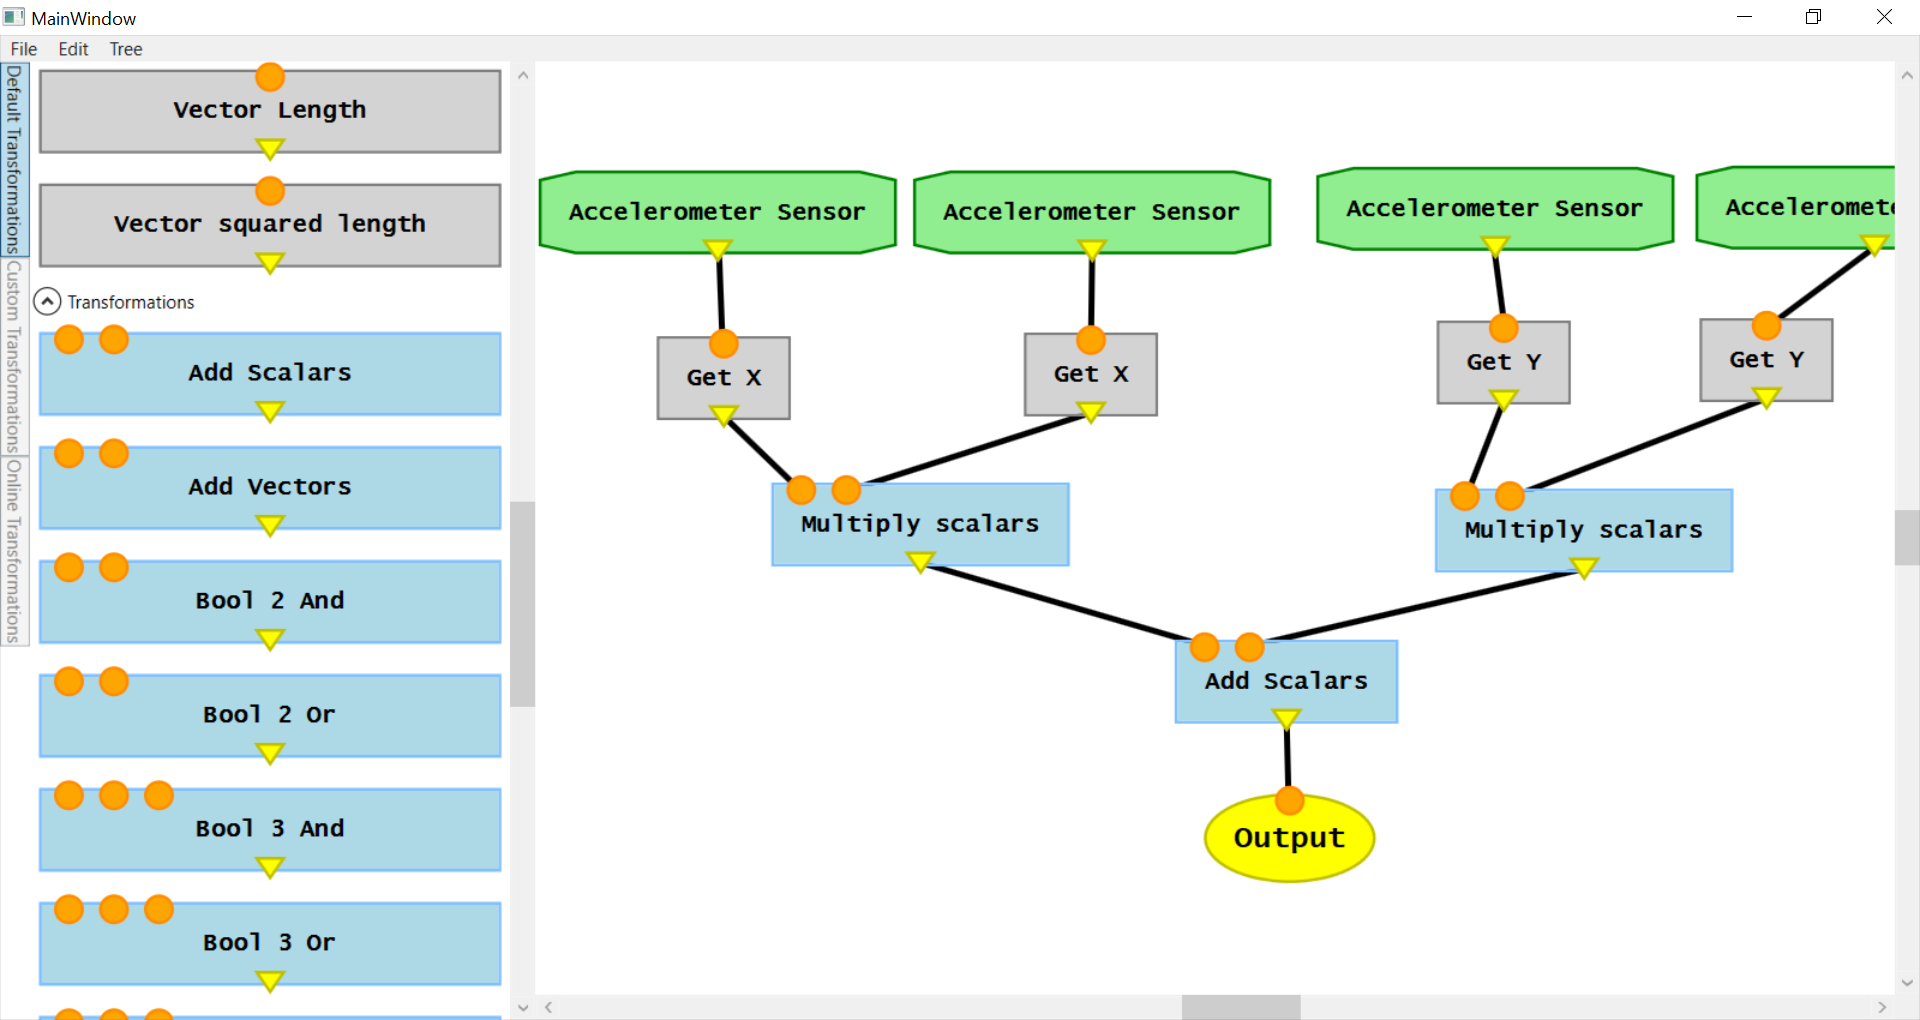
\includegraphics[width = \textwidth]{Screenshots/Smastra_0_0_alpha}
	\caption{Stand von SmaSTra in der Alpha Version}
	\label{fig:screenshot_0_0_alpha}
\end{figure}

\begin{itemize}
	\item welche Features sollten in der Alpha Version umgesetzt werden
	\item welche Features wurden tats\"achlich umgesetzt / was konnte die Alpha Version
	\item Feedback/Evaluation/Kritikpunkte der Alpha Version
\end{itemize}

\section{Weiterentwicklung der Alpha}

Die Alpha Version zeigte, dass das System umsetzbar war. Allerdings wurden auch etliche M\"angel deutlich, die den Umgang mit dem Tool erschwerten.
Un\"ubersichtlichkeit, fehlende Funktionalit\"aten und fehlendes visuelles Feedback waren mit die gr\"o{\ss}ten Kritikpunkte, die im Laufe der weiteren Entwicklung von SmaSTra behoben werden mussten.
\subsection{Neue Aufteilung der Nutzeroberfl\"ache}

\begin{figure} [h!]
	\centering
		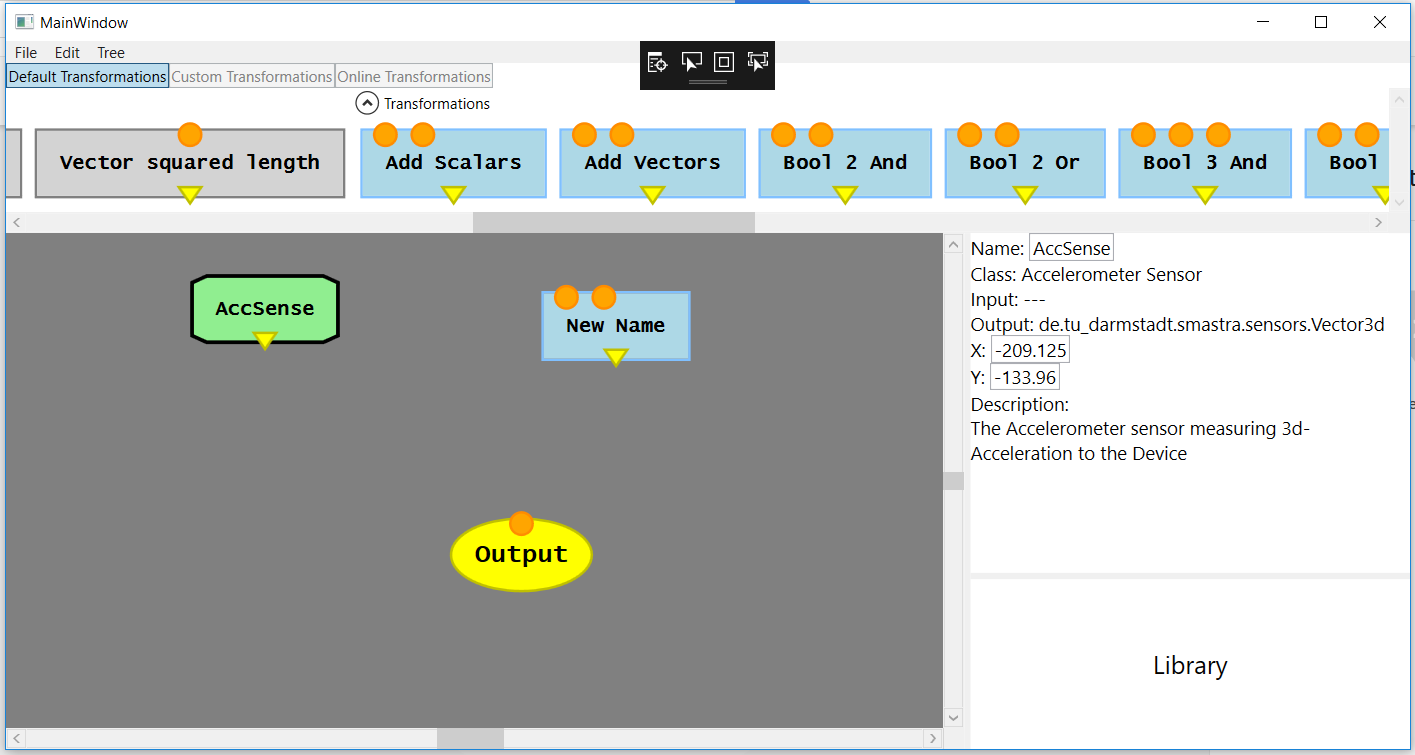
\includegraphics[width = \textwidth]{Screenshots/Smastra_0_2_properties}
	\caption{Aufteilung der GUI in Arbeitsfl\"ache, Obere Auswahlleiste, Properties und Library}
	\label{fig:screenshot_0_2_properties}
\end{figure}

Bei der Auswertung der Alpha Version zeigte sich, dass die bisherige Aufteilung der Nutzeroberfl\"ache den Anforderungen nicht gerecht wird. Daher wurden einige grundlegende \"anderungen eingef\"uhrt (vgl. Figure \ref{fig:screenshot_0_2_properties}).
Um einen besseren \"uberblick der zur verf\"ugung stehenden Elemente bieten zu k\"onnen, wurde die Elementauswahl in den gesamten oberen Bereich der Oberfl\"ache verlegt.
Entlang der rechten Seite wurden die zwei neue Bereiche Properties (oben) und Library (unten) hinzugef\"ugt. Im Properties Bereich k\"onnen die Details des aktuell ausgew\"ahlten Elements bearbeitet werden.
In der Library k\"onnen Elemente gespeichert werden, um so einen schnellen Zugriff auf h\"aufig verwendete Elemente zu gew\"ahrleisten.
Die gesamte restliche Fl\"ache wird als Hauptarbeitsbereich verwendet. 
\\

\subsection{Neue Repr\"asentation der Elemente}

\begin{figure} [h!]
	\centering
		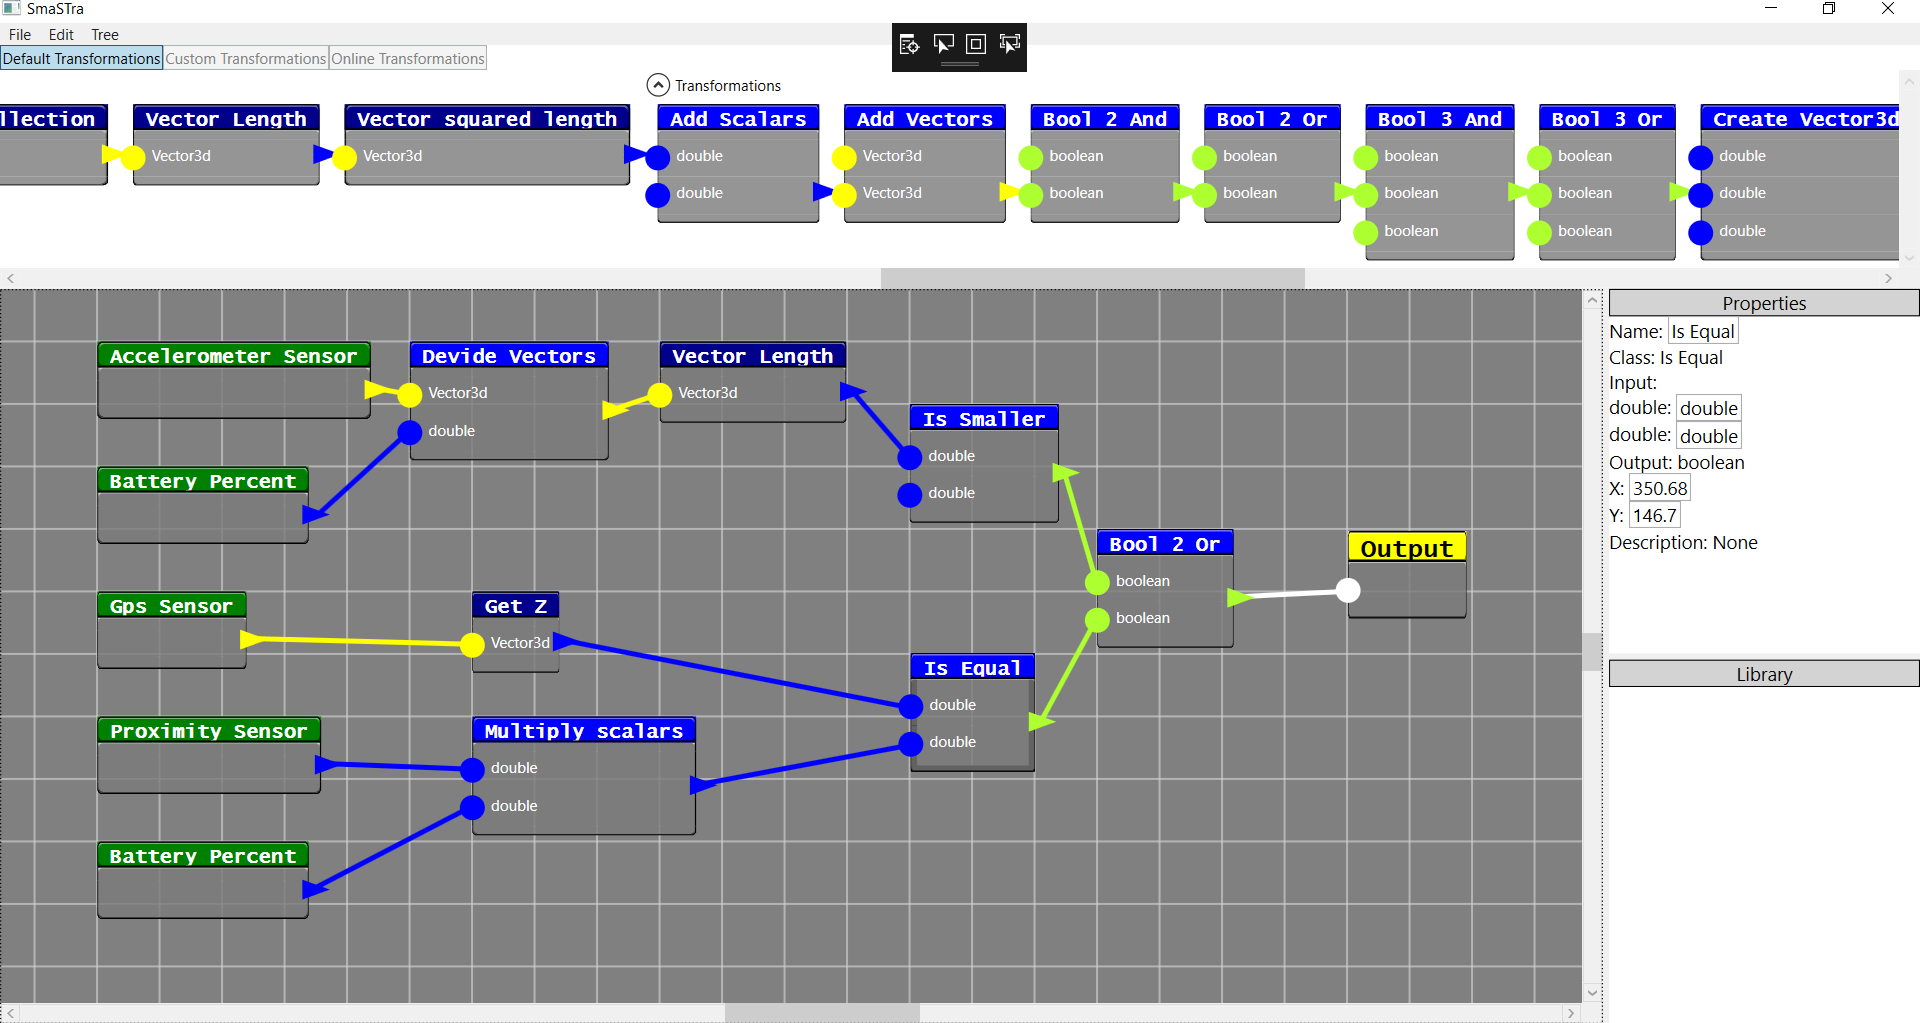
\includegraphics[width = \textwidth]{Screenshots/Smastra_0_5_new_generic_elements}
	\caption{Die Elemente wurden komplett \"uberarbeitet: Text und Farbe liefern Informationen zu den Eingabe- und Ausgabesockets. Der Arbeitsverlauf ist nun horizontal.}
	\label{fig:screenshot_0_5_new_generic_elements}
\end{figure}

Nachdem der grundlegende Aufbau der neuen Oberfl\"ache umgesetzt worden war, stand eine \"uberarbeitung der Elemente selbst an oberster Stelle (vgl. Figure \ref{fig:screenshot_0_5_new_generic_elements}).

Anstatt an der Ober- und Unterseite, sind die Sockets zur Ein- und Ausgabe nun seitlich an den Elementen angebracht. Dadurch verl\"auft die allgemeine Flussrichtung horizontal, wodurch die verf\"ugbare Fl\"ache des Hauptarbeitsbereiches besser genutzt werden kann. 
Zudem steht dadurch neben den Eingabesockets zus\"atzlicher Platz zur Verf\"ugung. Dieser wird genutzt, um den erwarteten Datentyp eines Eingabesockets anzuzeigen, solange an diesen noch kein Wert angelegt wurde. Sobald eine Verbindung an dem entsprechenden Socket angelegt oder ein Wert per Hand im Properties Bereich eingetragen wurde, wird, anstatt des Datentyps, der Name des verbundenen Elements bzw. der eingetragene Wert angezeigt.

S\"amtlichen Datentypen, die von den vorinstallierten Elementen genutzt werden, wurde jeweils eine bestimmte Farbe zugeordnet und alle Eingabe- und Ausgabesockets werden in der Farbe ihrer entsprechenden Datentypen dargestellt.
Auf diese Weise kann der Nutzer auf den erten Blick sehen, um welche Datentypen es sich handelt und ob diese miteinander verbunden werden k\"onnen.
\\

\subsection{Auswahlleiste und Men\"us}

\begin{figure}[h!]
	\centering
		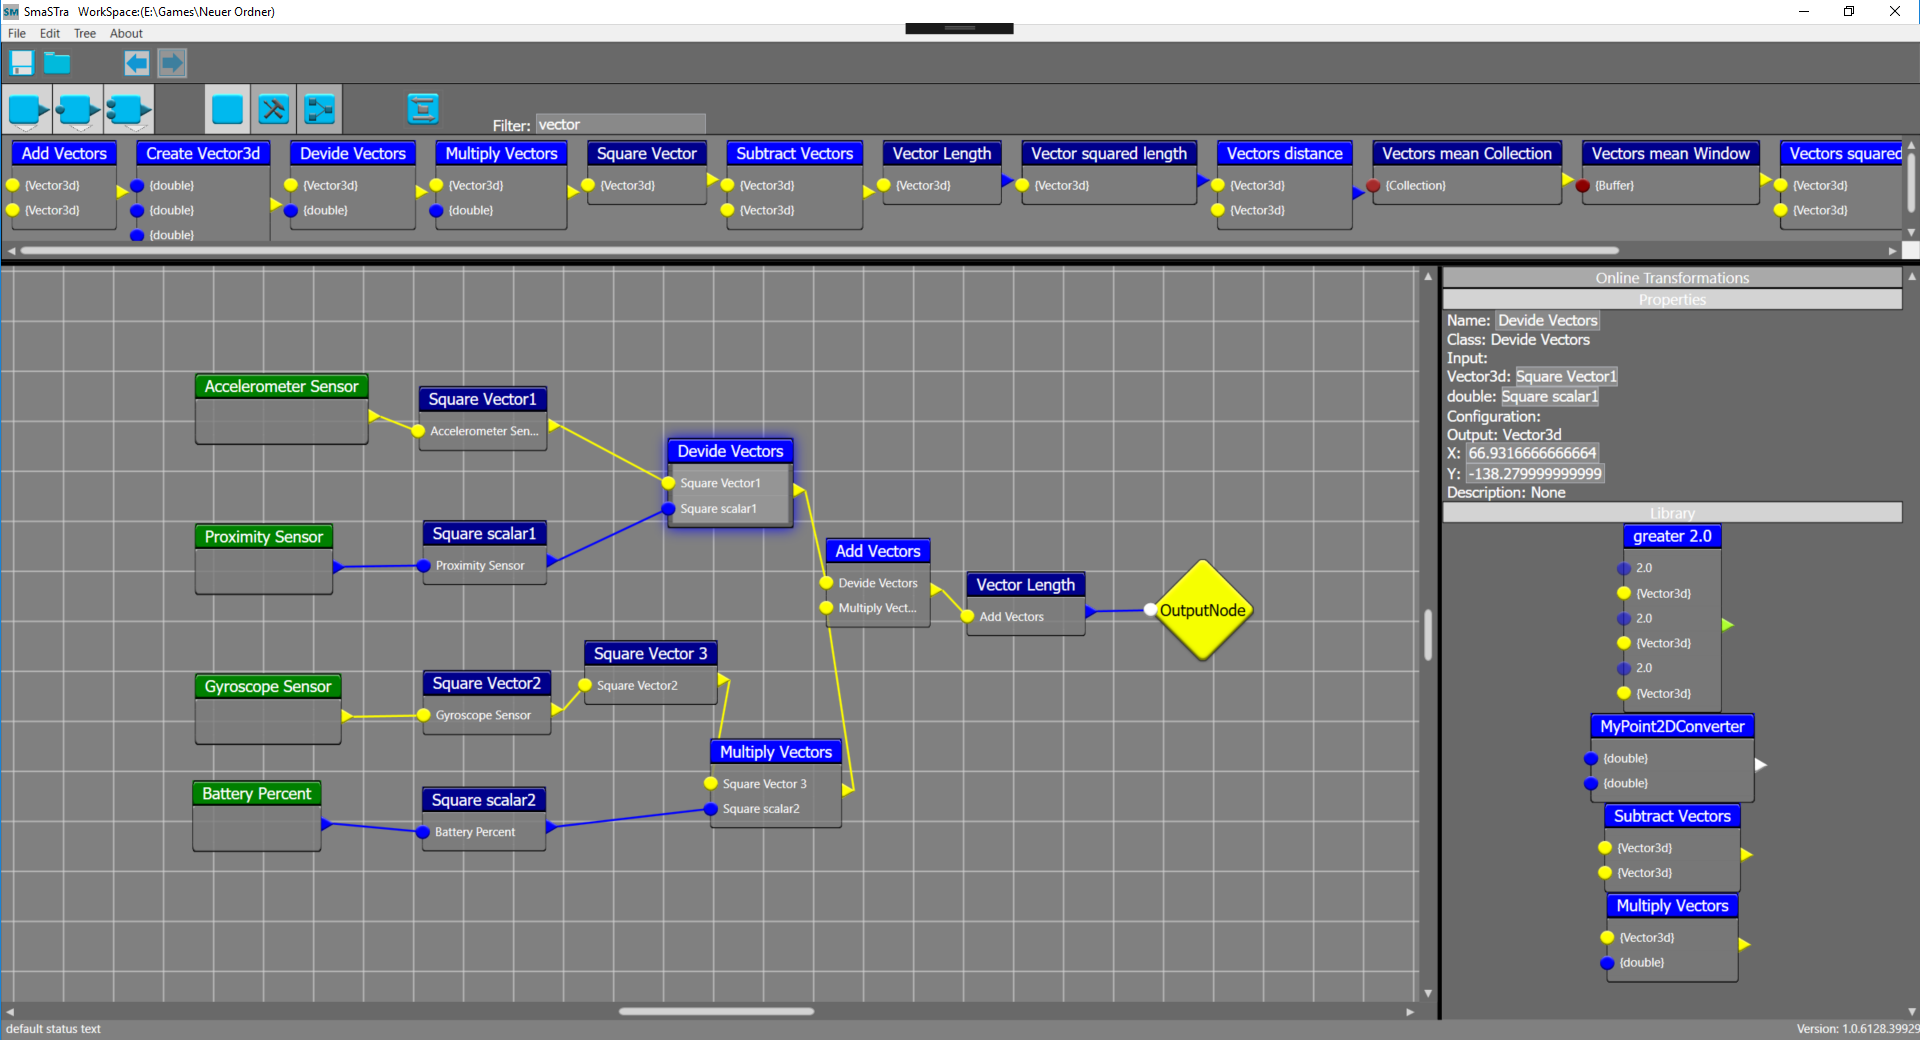
\includegraphics[width = \textwidth]{Screenshots/Smastra_1_4_filter_top_menu}
	\caption{Die Auswahlleiste verf\"ugt nun \"uber mehrere Filteroptionen um bestimmte Elemente schneller zu finden.}
	\label{fig:screenshot_1_4_filter_top_menu}
\end{figure}

Der Hintergrund der gesamten Nutzeroberfl\"ache wurde abgedunkelt. Dadurch stechen die farbigen Elemente markanter hervor und lenken somit die Aufmerksamkeit des Nutzers auf die wichtigeren Bereiche. Zudem ist das gew\"ahlte Farbthema bei l\"angeren Arbeiten schonender f\"ur die Augen als eine grelle Arbeitsoberfl\"ache.

Zur effektiveren Handhabung der Vielzahl an unterschiedlichen Elementen, wurden weitere Kategorien eingef\"uhrt nach denen die Elemente gefiltert werden k\"onnen.
Diese Kategorien unterscheiden zum einen nach der Anzahl der Eingabewerte und zum anderen danach, ob das Element von Nutzern erstellt wurde oder bereits vorinstalliert war.
Zudem erlaubt ein Eingabefeld das Filtern nach beliebigen Stichw\"ortern, um so schnell Elemente aufzulisten, die thematisch zusammen geh\"oren.

Diese Filteroptionen wurden zusammen mit h\"aufig verwendeten Funktionen in einer Men\"uleiste entlang des oberen Randes der Nutzeroberfl\"ache platziert, so dass sie jederzeit sichtbar und schnell erreichbar sind. Au{\ss}erdem wurden eine Reihe von Tastenk\"urzeln und Kontextmen\"us eingef\"uhrt, die dem Nutzer das Navigieren \"uber die Arbeitsfl\"ache und das Arbeiten mit den Elementen erleichtert.

\chapter{SmaSTra Bedienungsanleitung}

\section{Was ist SmaSTra?}



\section{Beispielanwendung}

In diesem Abschnitt werden die grundlegenden Funktionen von SmaSTra anhand eines einfachen Anwendungsbeispiels gezeigt. 
In diesem Beispiel wird ein Sensor erstellt, der ausgeben soll, ob ein Ger\"at (beispielsweise ein Smartphone) schnell in eine beliebige Richtung beschleunigt wird.
Zu diesem Zweck soll \"uberpr\"uft werden, ob einer der Ausgabewerte des "Linear Accelerometer Sensors" einen bestimmten Schwellenwert \"uberschreitet.

\paragraph{Elemente ausw\"ahlen}

\begin{figure}[h!]
	\centering
		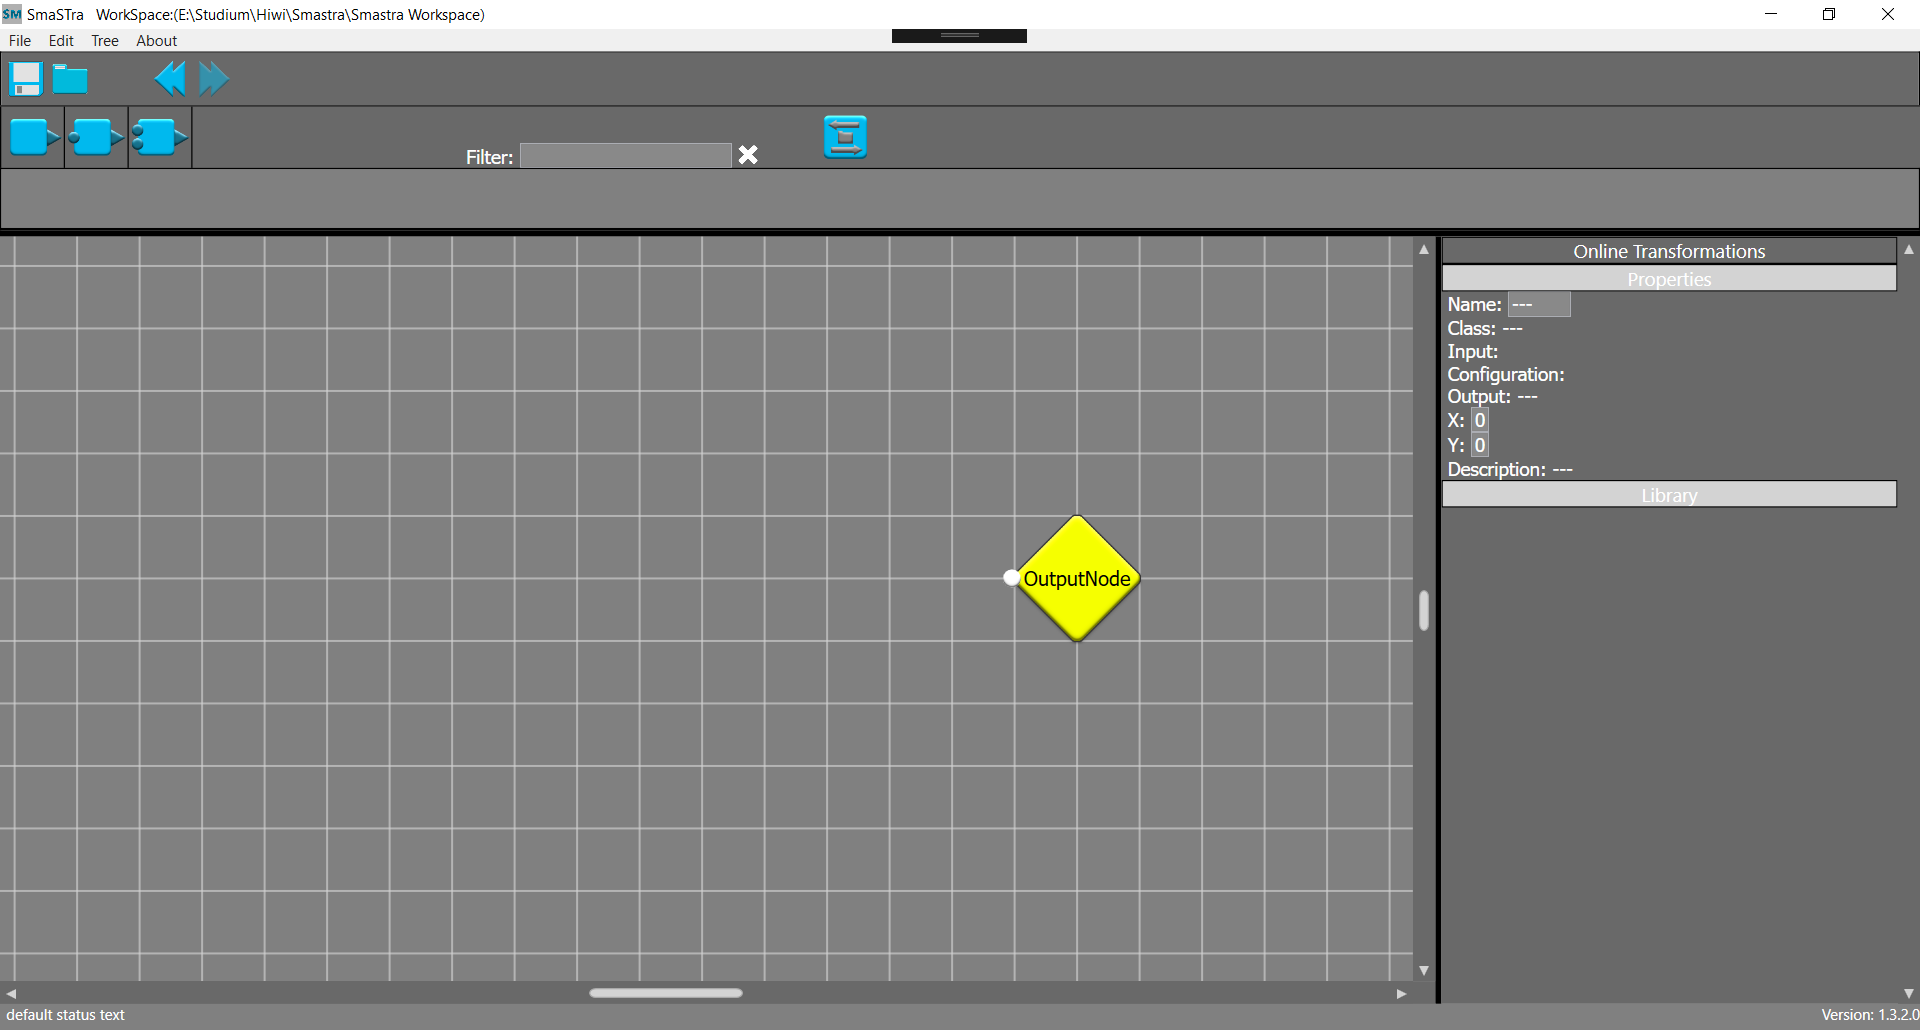
\includegraphics[width = \textwidth]{Manual/01_startup}
	\caption{Der Hauptbildschirm direkt nach dem Start von SmaSTra}
	\label{fig:manual_01_startup}
\end{figure}

Nach dem Starten von SmaSTra und der Anzeige des Splashscreen, erscheint der Hauptbildschirm (vgl. Figure \ref{fig:manual_01_startup}). Im Arbeitsbereich befindet sich nur das Output-Element.
\\
Nun soll zun\"achst ein "Linear Accelerometer Sensor" in den Arbeitsbereich gezogen werden. Mit einem Klick auf die Schaltfl\"ache "Data Sources" 
\includegraphics[width = 20pt]{Manual/datasources}, werden diejenigen vorinstallierten Elemente angezeigt, die als Datenquellen dienen. Per Drag\&Drop kann der Linear Accelerometer Sensor im Arbeitsbereich platziert werden, am besten in der N\"ahe des linken Randes.
\\
Anhand der Farbe und des Tooltips des Ausgabesockets kann man ablesen, dass der Ausgabetyp des Linear Accelerometer Sensor ein 3-dimensionaler Vektor ist. Jede Komponente des Vektors gibt die Beschleunigung in eine bestimmte Richtung an (vor/zur\"uck, links/rechts, hoch/runter). Um mit dem Wert einer einzelnen Komponente des Vektors arbeiten zu k\"onnen, wird ein weiteres Element ben\"otigt. Mit einem Klick auf die Schaltfl\"ache "Conversions" 
\includegraphics[width = 20pt]{Manual/conversions} werden auch diejenigen Elemente angezeigt, die einen einzelnen Eingabewert erwarten.
Suchen Sie das Element "Get X" und platzieren Sie es rechts neben dem Linear Accelerometer Sensor. Wie man an der Farbe des Eingabesocket von Get X erkennen kann, wird hier ein 3-dimensionaler Vektor erwartet. Der Ausgabesocket des Linear Accelerometer Sensors kann also mit dem Eingabesocket von Get X verbunden werden.

\paragraph{Elemente Verbinden}

\begin{figure}[h!]
	\centering
		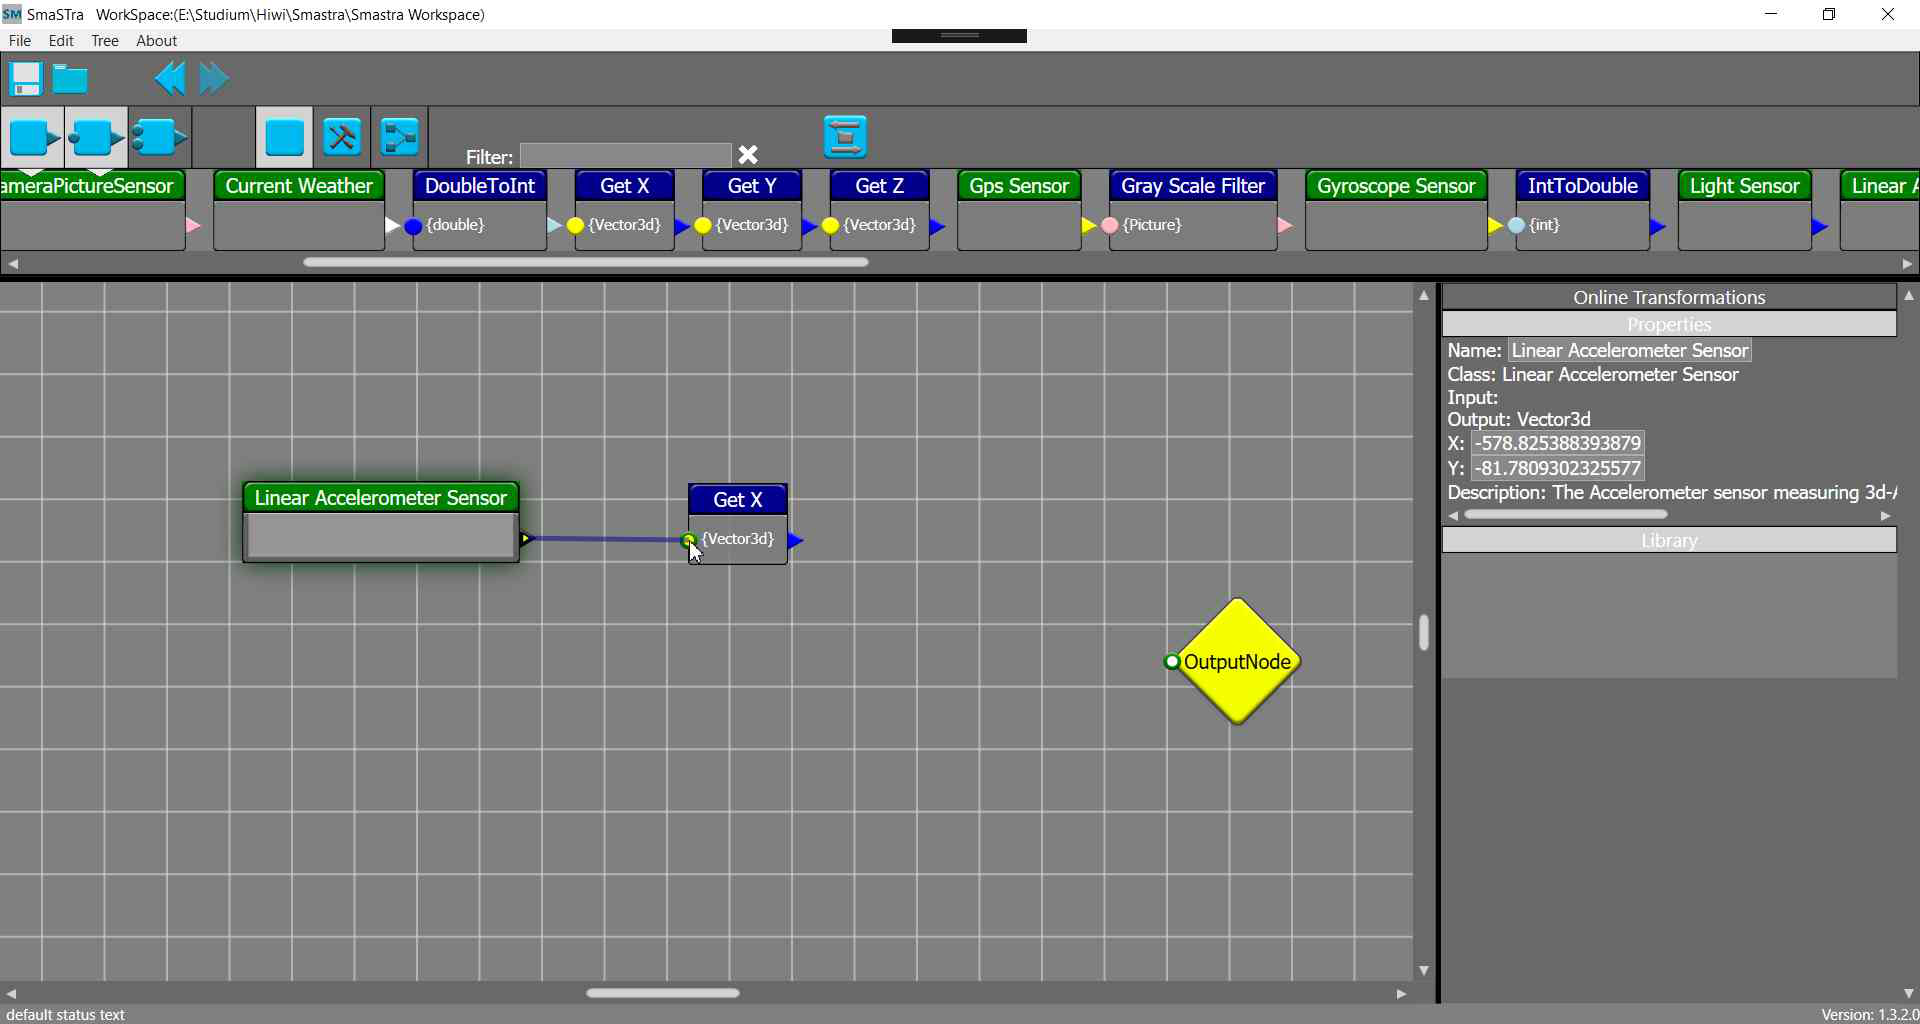
\includegraphics[width = \textwidth]{Manual/05_dragging_connection}
	\caption{Verbinden des Linear Accelerometer Sensors mit Get X}
	\label{fig:manual_05_dragging_connection}
\end{figure}

Um eine Verbindung zwischen zwei kompatiblen Elementen herzustellen, klicken und halten sie einen der beiden Sockets gedr\"uckt und bewegen Sie die Maus bei gedr\"uckter Maustaste. Eine dunkelblaue Verbindungslinie erscheint zwischen ihrer Maus und dem gehaltenen Socket. Au{\ss}erdem erscheint um s\"amtliche kompatiblen Sockets ein gr\"uner Rand, w\"ahrend inkompatible Sockets rot umrandet werden (vgl. Figure \ref{fig:manual_05_dragging_connection}). Bewegen Sie nun die Maus \"uber den Socket mit dem Sie eine Verbindung aufbauen m\"ochten und lassen Sie die Maustaste los. Eine Linie verbindet nun dauerhaft die beiden Elemente. Die Farbe der Linie entspricht dabei der Farbe der Datentypen der Sockets. Zus\"atzlich wird neben dem Eingabesocket der Name des Verbundenen Elements angezeigt (in diesem Fall Linear Accelerometer Sensor). Die Ausgabe von Get X ist vom Typ double und entspricht in diesem Fall der Beschleunigung des Smartphones entlang der X-Achse.

\paragraph{Werte per Hand eintragen}

\begin{figure}[h!]
	\centering
		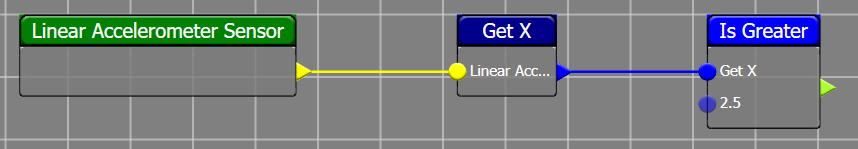
\includegraphics[width = \textwidth]{Manual/08_enter_value_cut}
	\caption{Der Wert des unteren Eingabesockets von Is Greater wurde per Hand auf 2.5 gesetzt}
	\label{fig:08_enter_value_cut}
\end{figure}

Als n\"achstes soll verglichen werden, ob die Beschleunigung entlang der X-Achse einen bestimmten Schwellenwert \"uberschreitet. F\"ur dieses Beispiel w\"ahlen wir einen Wert von $2.5m/s^2$. F\"ur den Vergleich wird das Element "Is Greater" verwendet. Mit einem Klick auf die Schaltfl\"ache "Transformations" 
\includegraphics[width = 20pt]{Manual/transformations} werden auch diejenigen Elemente angezeigt, die mehr als einen Eingabewert erwarten. Ziehen Sie Is Greater in den Arbeitsbereich rechts neben Get X und verbinden Sie den Ausgabesocket von Get X mit dem oberen Eingabesocket von Is Greater. Da wir den Schwellenwert selbst auf 2.5 festlegen und er von keinen anderen Elementen abh\"angt, k\"onnen wir diesen Wert per Hand eintragen. Mit einem Doppelklick auf den unteren Eingabesocket von Is Greater werden die Details dieses Elements im "Properties" Bereich am rechten Rand angezeigt. Unter "Inputs" werden f\"ur beide Eingabesockets jeweils der erwartete Datentyp (double) und der aktuell angelegte Wert angegeben. Als Wert des oberen Sockets wird der Name des verbundenen Elements angezeigt (Get X). Der Wert des unteren Sockets ist noch leer, da noch kein Wert angegeben wurde. In dieses leere Feld kann nun der Wert von 2.5 eingetragen werden. Durch das Eintragen eines Wertes per Hand wird im Is Greater Element der entsprechende Eingabesocket transparent und der entsprechende Wert erscheint neben dem Socket (vgl. Figure \ref{fig:08_enter_value_cut}).

\paragraph{Kopieren und Filtern von Elementen}

\begin{figure}[h!]
	\centering
		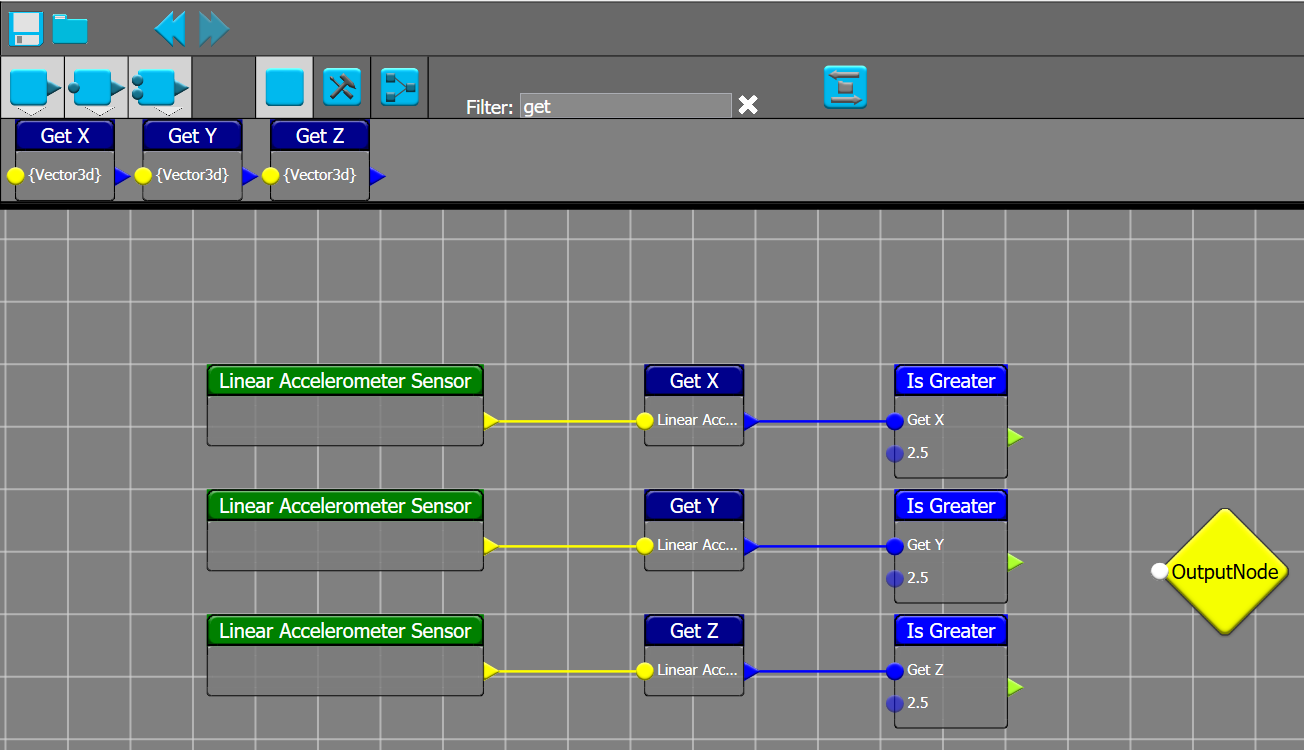
\includegraphics[width = \textwidth]{Manual/09_filter}
	\caption{Weitere Linear Accelerometer Sensoren und Is Greater Elemente wurden durch Kopieren hinzugef\"ugt. Die Auswahlleiste wird nach "get" gefiltert}
	\label{fig:09_filter}
\end{figure}

Nun sollen auch Bewegungen in Y- und Z-Richtung erkannt werden. Zu diesem Zweck werden je zwei weitere Linear Accelerometer Sensoren und Is Greater Elemente ben\"otigt.
Anstatt diese Elemente aus der oberen Auswahlleiste heraus zu ziehen, k\"onnen Elemente, die sich bereits im Arbeitsbereich befinden, auch direkt kopiert werden. 
W\"ahlen Sie den Linear Accelerometer Sensor im Arbeitsbereich mit einem Linksklick aus. F\"ugen Sie dann Is Greater mit Strg+Linksklick zur Auswahl hinzu. Mit Strg+V wird nun von beiden Elementen jeweils eine Kopie erstellt. Ziehen Sie die Kopien ein St\"uck nach unten und kopieren Sie sie erneut. Der in Is Greater eingetragene Wert bleibt dabei erhalten.
Als n\"achstes werden die zwei Elemente Get Y und Get Z ben\"otigt. Die Auswahlleiste d\"urfte inzwischen eine Vielzahl unterschiedlicher Elemente anzeigen. Um Get Y/Z schnell zu finden, kann der Filter verwendet werden. Geben Sie in das Eingabefeld des Filters "Get" ein, um alle Elemente anzuzeigen, die diese Zeichenfolge in ihrem Namen haben (vgl. Figure\ref{fig:09_filter}). Stellen Sie sicher, dass dabei die Schaltfl\"ache f\"ur Conversions aktiv ist. Nun k\"onnen Get Y und Get Z in die Arbeitsfl\"ache gezogen und analog zu Get X mit den Kopien des Linear Accelerometer Sensors und Is Greater verbunden werden. Leeren Sie den Filter anschlie{\ss}end wieder, um alle Elemente anzeigen zu lassen.
\\

\begin{figure}[h!]
	\centering
		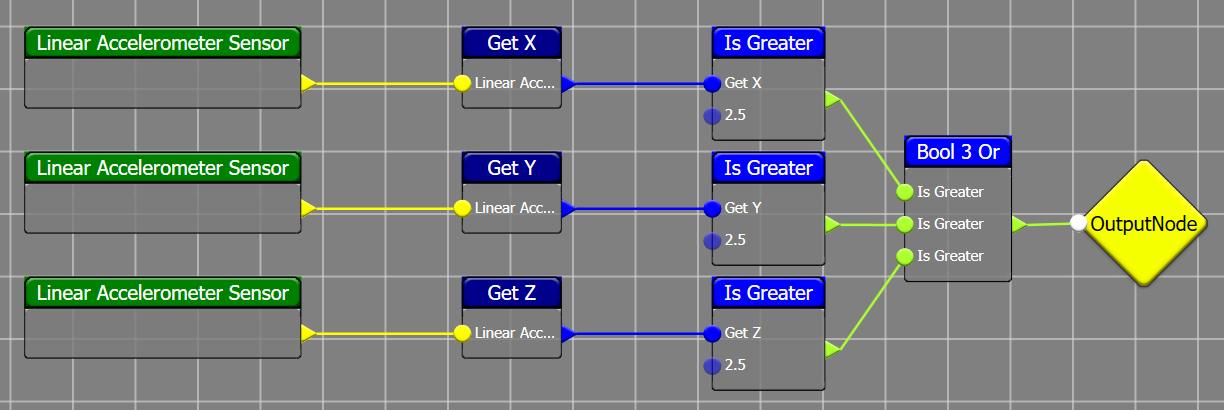
\includegraphics[width = \textwidth]{Manual/10_first_test}
	\caption{Alle Elemente sind durch Bool 3 Or mit dem Output verbunden. Der Java Code kann generiert werden}
	\label{fig:10_first_test}
\end{figure}

Abschlie{\ss}end m\"ussen die drei erstellten Zweige noch korrekt zusammengef\"uhrt werden. Da als Ergebnis "true" ausgegeben werden soll, wenn einer der Zweige "true" ergibt, m\"ussen diese mit einer Or-Verkn\"upfung verbunden werden. In den Transformations findet sich daf\"ur das Element "Bool 3 Or". Ziehen Sie es in den Arbeitsbereich links neben Output.
Verbinden Sie die Ausgabesockets der Is Greater Elemente mit jeweils einem Eingabesocket von Bool 3 Or und dessen Ausgabesocket mit dem Output. Der Arbeitsbereich sollte aktuell \"ahnlich aussehen wie in Figure \ref{fig:10_first_test}.

\paragraph{Erstellen einer Java Klasse}
Nun ist es an der Zeit f\"ur den ersten Testlauf. In diesem Anwendungsbeispiel, wird davon ausgegangen, dass der von SmaSTra generierte Code in einem Android Studio
Projekt verwendet werden soll. Eine Beschreibung zur Exportierung des Codes in andere Entwicklungsumgebungen, wie zum Beispiel Eclipse, findet sich in Abschnitt \ref{sub:Generate}.
\\
Erstellen Sie ein neues Android Studio Projekt, falls noch kein Projekt existiert, mit dem Sie SmaSTra testen wollen. Klicken Sie in SmaSTra in der oberen Men\"uleiste auf "Tree" und w\"ahlen Sie die Option "Generate Java code...". Navigieren Sie zu ihrem Android Studio Projekt und w\"ahlen dort den Ordner "app" als Speicherort aus. Geben Sie den Namen ein, den die neue Java Klasse erhalten soll (in diesem Beispiel nennen wir sie "MovementSensor") und klicken Sie anschlie{\ss}end auf "Speichern". Wenn das Android Studio Projekt korrekt erkannt wurde, bittet ein Dialog um Erlaubnis, um den generierten Code automatisch in das gew\"ahlte Projekt zu integrieren. Best\"atigen Sie und klicken im anschlie{\ss}enden Dialog auf "Ok".
\\
Starten Sie Android Studio, falls nicht schon geschehen, und \"offnen Sie das Projekt, in das gerade der SmaSTra Code exportiert wurde. W\"ahlen Sie "Tools" in der oberen Men\"uleiste, dort auf Android und anschlie{\ss}end auf "Sync Project with Gradle Files". Sobald die Synchronisation abgeschlossen ist, kann die MovementSensor Klasse in ihrem eigenen Code verwendet werden. 
\\
Erstellen Sie daf\"ur eine Instanz von MovementSensor und rufen Sie auf ihr die Methode start() auf. Ab jetzt kann der Wert des in SmaSTra gebauten MovementSensor einfach durch die Methode getData() abgefragt werden. Der Code in Figure \ref{fig:firstcodeTest} zeigt ein Beispiel, wie die Ausgabe des MovementSensor \"uberpr\"uft werden kann. 
F\"ugen Sie den Code in die onCreate Methode ihrer MainActivity mit ein und testen Sie das Programm auf einem angeschlossenen Smartphone oder Tablet. Die Ausgabe in der Konsole sollte durchgehend "false" ausgeben, solange das Ger\"at nur wenig bewegt wird. Aber auch bei schnellen Bewegungen scheint die Ausgabe nicht immer auf "true" zu wechseln. Genauere Tests zeigen, dass der MovementSensor nur dann korrekt "true" ausgibt, wenn das Ger\"at schnell genug nach rechts, oben oder auf den Nutzer zu bewegt wird. Bewegungen nach links, unten und vom Nutzer weg, werden noch nicht richtig erkannt. Diesem Problem widmet sich der n\"achste Abschnitt.
\\

\begin{figure}[h!]
\begin{lstlisting}
@Override
    protected void onCreate(Bundle savedInstanceState) {
        super.onCreate(savedInstanceState);
        setContentView(R.layout.activity_main);

        final MovementSensor myMovementSensor = new MovementSensor(this);
        myMovementSensor.start();

        Timer timer = new Timer();
        timer.schedule(new TimerTask() {
            @Override
            public void run() {
               Log.d("SmaSTra Test", "Device is Moving: " + myMovementSensor.getData());
            }
        }, 1000, 1000);
    }
\end{lstlisting}
\caption{Java Code zum Testen der in SMaSTra erstellten MovementSensor Klasse}%
\label{fig:firstcodeTest}
\end{figure}

\paragraph{Erstellen von Custom Elementen}
\begin{figure}[h!]
	\centering
		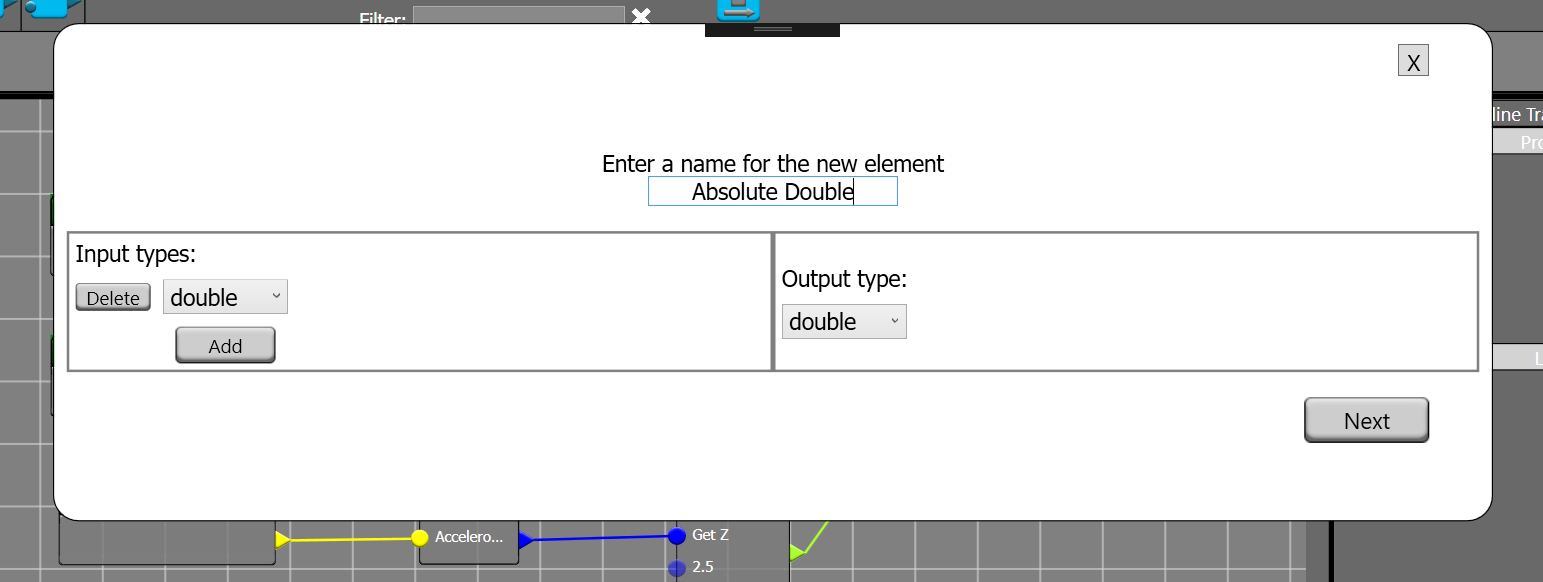
\includegraphics[width = \textwidth]{Manual/11_custom_name}
	\caption{Erste Seite zum erstellen eines eigenen Elements. Hier werden der Name sowie Eingabe- und Ausgabetypen festgelegt}
	\label{fig:11_custom_name}
\end{figure}

\begin{figure}[h!]
	\centering
		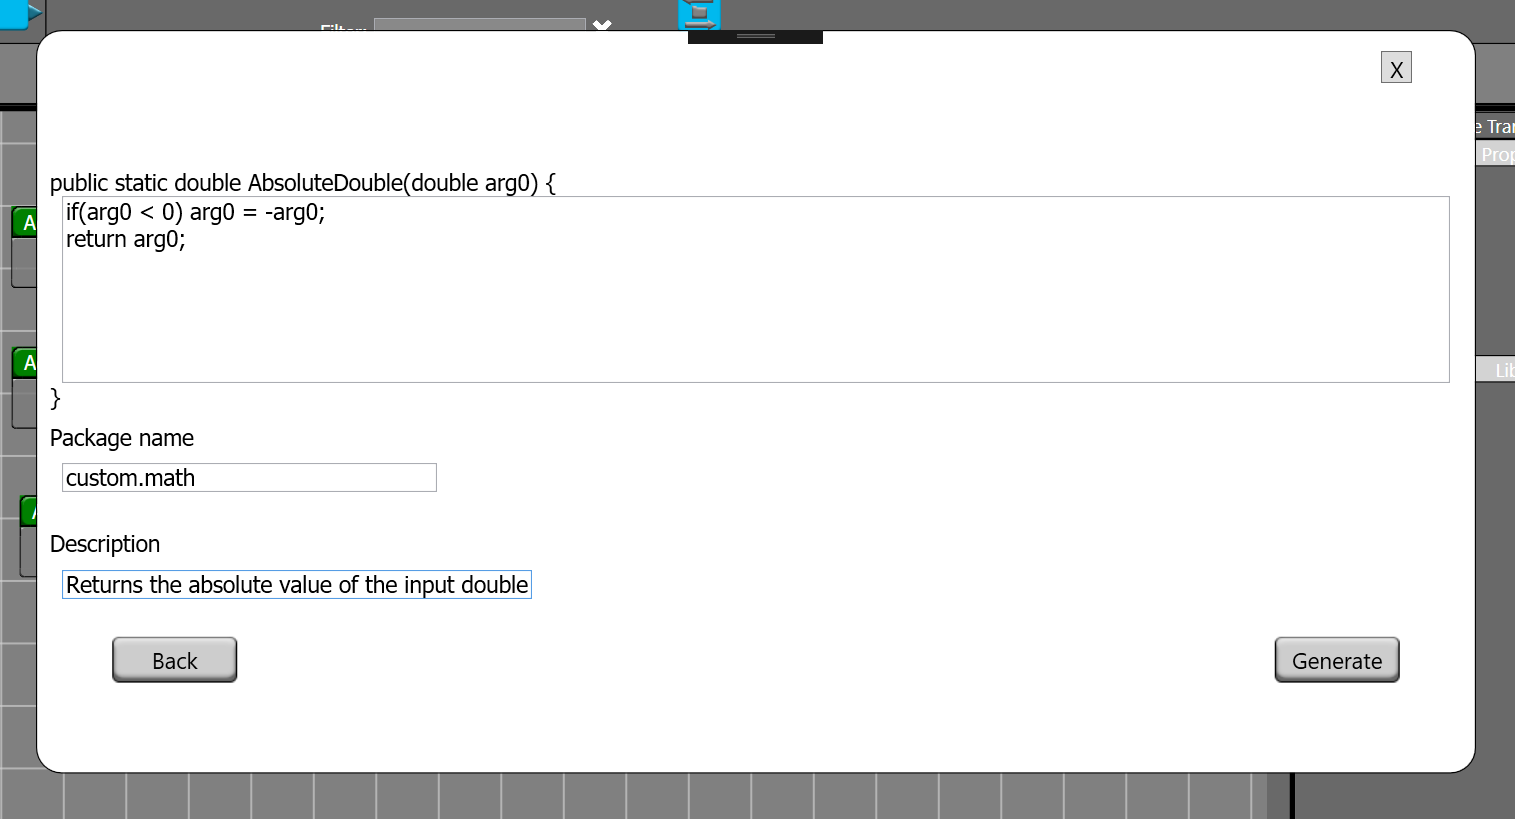
\includegraphics[width = \textwidth]{Manual/12_custom_code}
	\caption{Zweite Seite zum erstellen eines eigenen Elements. Hier werden der auszuf\"uhrende Code, Packagename und Beschreibung eingegeben }
	\label{fig:12_custom_code}
\end{figure}

Ein Linear Accelerometer Sensor gibt f\"ur jede der drei Richtungsachsen X,Y und Z einen Wert aus. Bewegt sich das Ger\"at in positiver Richtung entlang einer Achse (z.b. nach rechts im Fall der X-Achse), wird auch ein positiver Wert ausgegeben. Eine Bewegung in negativer Richtung f\"uhrt zu einem negativen Wert.
Der bisher erstellte Java Code reagiert jedoch nur auf positive Werte, da negative Werte niemals den Schwellenwert von 2.5 \"uberschreiten k\"onnen.
\\
Eine m\"ogliche L\"osung w\"are es, alle bisher verwendeten Elemente zu kopieren, anstatt Is Greater das Element Is Smaller mit einem Wert von -2.5 zu verwenden und die beiden Teilb\"aume mit einem Bool 2 Or zu verbinden.
Allerdings gibt es auch eine elegantere L\"osung. Daf\"ur wird ein Element ben\"otigt, dass eine potenziell negative Ausgabe von Get X/Y/Z in einen positiven Wert umwandelt.
Ein solches Element findet sich allerdings nicht in der Auswahlliste, daher muss es vom Nutzer selbst erstellt werden. \"Uber "Edit" und anschlie{\ss}end "Create Custom Element" erscheint das Fenster zum erstellen eigener Elemente. Hier kann zun\"achst der Name des Elements, sowie seine Eingabe- und Ausgabetypen  festgelegt werden (vgl. Figure \ref{fig:11_custom_name}). In diesem Beispiel wird das Element "Absolute Double" genannt. Als Eingabe- bzw. Ausgabetypen wird jeweils "double" verwendet. Mit einem Klick auf "Next" gelangt man zur n\"achsten Seite.
Hier kann nun der Java/Android Code eingegeben werden, den das Element ausf\"uhren soll. Der Methodenkopf ist bereits vorgegeben. Der Eingabeparameter "arg0" soll in eine positive Zahl umgewandelt werden, falls er negativ ist. Der Code w\"are demnach beispielsweise:
\\
\\
if(arg0 < 0) arg0 = -arg0;
\\
return arg0; 
\\
\\
Geben Sie anschlie{\ss}end noch einen beliebigen Packagenamen und eine Beschreibung des Elements an und Klicken Sie auf "Generate" (vgl. Figure \ref{fig:12_custom_code}). Dadurch wird eine neu Conversion erstellt, und der Auswahlleiste hinzugef\"ugt. Bisher werden allerdings vorinstallierte Elemente angezeigt. Mit einem Klick auf die Schaltfl\"ache "Custom Elements" 
\includegraphics[width = 15pt]{Manual/custom_elements} werden auch Elemente angezeigt, die vom Nutzer selbst erstellt wurden. Das neue Element Absolute Double sollte nun auch bei den Conversions auftauchen. Schalten Sie je ein Absolute Double Element zwischen Get X/Y/Z und Is Greater. Sollte der Arbeitsbereich un\"ubersichtlich werden, kann er jederzeit durch die Tastenkombination Strg+F geordnet werden (vgl. Figure \ref{fig:13_organize}). 
Anschlie{\ss}endes Generieren und Testen der Java Klasse zeigt, dass die Klasse genau dann "true" ausgibt, wenn das Ger\"at stark in beliebiger Richtung beschleunigt wird, was genau dem gew\"unschten Verhalten entspricht.

\begin{figure}[h!]
	\centering
		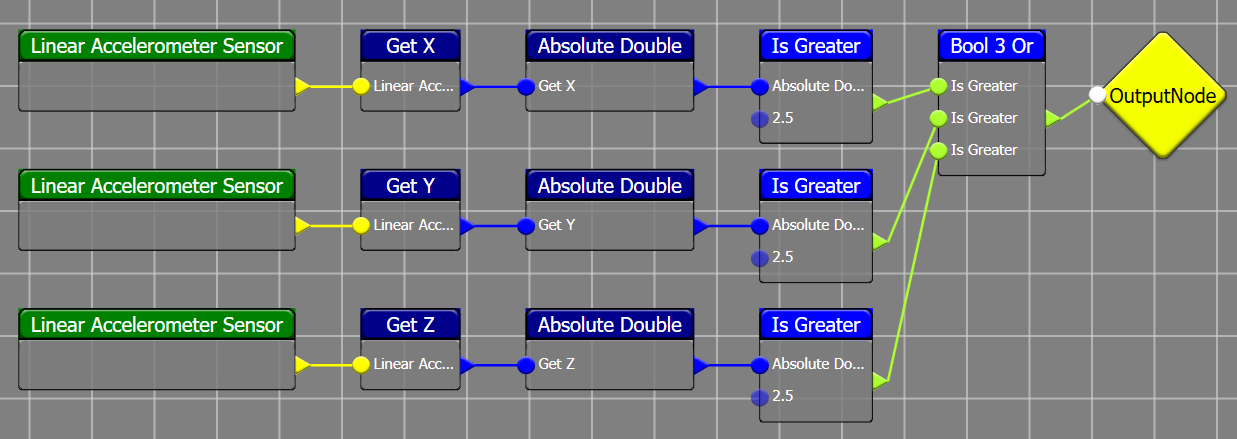
\includegraphics[width = \textwidth]{Manual/13_organize}
	\caption{Arbeitsbereich nach dem Hinzuf\"ugen von Absolute Double und anschlie{\ss}endem Ordnen}
	\label{fig:13_organize}
\end{figure}


\paragraph{Erstellen von Combined Elementen}

\begin{figure}[h!]
	\centering
		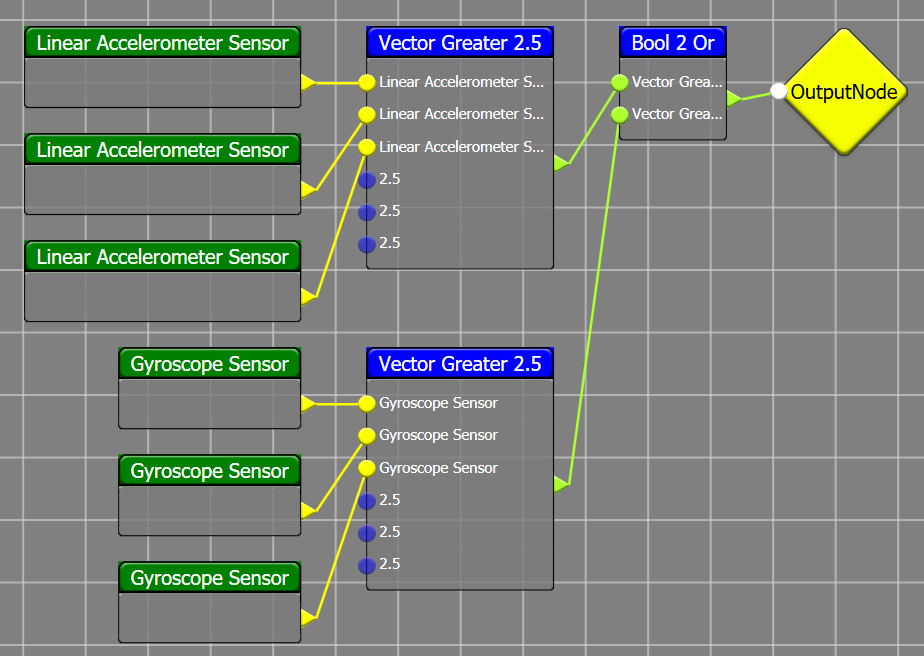
\includegraphics[width = \textwidth]{Manual/14_combined}
	\caption{Arbeitsbereich nach Erstellen von Vector Greater 2.5 und Verbinden beider Zweige mit Output}
	\label{fig:14_combined}
\end{figure}

Das obige Beispiel soll nun noch erweitert werden, um auch auf Rotation zu reagieren. Zus\"atzlich zum bisherigen Verhalten soll die generierte Java Klasse auch dann "true" ausgeben, wenn das Ger\"at mit mehr als $2.5 rad/s$ um eine beliebige Achse rotiert. Diese Aufgabe ist der vorangegangenen sehr \"ahnlich und auch die ben\"otigten Elemente sind fast identisch. Ein L\"osungsansatz w\"are es, einfach jedes einzelne Element zu kopieren und damit einen zweiten Baum zu erstellen, bei dem die drei Linear Accelerometer Sensoren durch Gyroscope Sensoren ersetzt werden. Diese Vorgehensweise ist zwar prinzipiell korrekt, f\"uhrt aber zu einer hohen Anzahl redundanter Elemente.
\\
Doch anstatt jedes Element einzeln zu kopieren, ist es m\"oglich eine Gruppe von verbundenen Elementen zu einem einzelnen Element zusammenzufassen. Ziehen Sie mit der linken Maustaste einen Rahmen um alle Elemente, ausgenommen dem Output und den drei Linear Accelerometer Sensoren. Klicken Sie dann mit der rechten Maustaste auf eines der markierten Elemente und w\"ahlen Sie im Kontext Men\"u "Merge current selection". Geben Sie in dem erscheinenden Fenster einen Namen f\"ur das neue Element an (in diesem Beispiel wird es "Vector Greater 2.5" genannt) und best\"atigen Sie mit "OK". Aus den zuvor markierten Elementen wurde nun ein einzelnes Element generiert. Elemente die auf diese Weise erstellt werden, befinden sich in der Auswahlleiste in einer eigenen Kategorie. Klicken Sie auf die Schaltfl\"ache "Combined Elements" 
\includegraphics[width = 15pt]{Manual/combined_transf} um diese Elemente anzeigen zu lassen. Ziehen Sie ein zweites Vector Greater 2.5 Element zusammen mit drei Gyroscope Sensoren in den Arbeitsbereich. Verbinden Sie die Gyroscope Sensoren mit dem zweiten Vector Greater 2.5 analog zu den Linear Accelerometer Sensoren. Abschlie{\ss}end wird noch ein "Bool 2 Or" ben\"otigt. Verbinden Sie dieses mit den jeweiligen Ausgabesockets der beiden Vector Greater 2.5 und dem Output (vgl. Figure \ref{fig:14_combined}).
Damit ist schon die n\"achste Java Klasse bereit, um erstellt und getestet zu werden. Wie gew\"unscht sollte nun auch bei einer entsprechend hohen Rotationsgeschwindigkeit des Ger\"ats "true" ausgegeben werden.



\section{Einzelanleitung zu jeder Funktion}

\subsection{}

\subsection{Auswahlleiste} \label{sub:Auswahlleiste}
Die Auswahlleiste beinhaltet s\"amtliche Elemente, die im akutellen Workspace gespeichert sind. Im Regelfall sind dies alle vorinstallierten Elemente, sowie den vom Nutzer erstellten eigenen Elementen und den kombinierten Elementen. Um Elemente besser einordnen zu k\"onnen, werden sie jeweils nach zwei Kriterien unterschieden.
Das erste ist die Anzahl ihrer Eingabesockets. Elemente ohne ein Eingabesocket werden als "Datasources" bezeichnet. Elemente mit genau einem Eingabesocket sind "Conversions" und mit mehr als einem Eingabesocket sind "Transformations". Mit den jeweiligen Schaltfl\"achen oberhalb der Auswahlleiste lassen sich die Datasources 
\includegraphics[width = 20pt]{Manual/datasources}, Conversions 
\includegraphics[width = 20pt]{Manual/conversions} und Transformations 
\includegraphics[width = 20pt]{Manual/transformations} in der Auswahlleiste ein und ausblenden.
\\
Das zweite Kriterium ist die Art wie das jeweilige ELement erstellt wurde. Vorinstallierte Elemente werden als "Default Elements" bezeichnet, vom Nutzer erstellte Elemente sind "Custom Elements" und zusammengefasste Elemente werden als "Combined Elements" bezeichnet. Auch hier k\"onnen Elemente einer bestmmten Kategorie mit den Schaltfl\"achen Default Elements 
\includegraphics[width = 15pt]{Manual/default_transf}, Custom Elements 
\includegraphics[width = 15pt]{Manual/custom_elements} und Combined Elements 
\includegraphics[width = 15pt]{Manual/combined_transf} ein oder ausgeblendet werden.
\\
Zus\"atzlich zu den beiden Kriterien, kann auch nach den Namen der Elemente gefiltert werden. Sobald eine Zeichenfolge in das "Filter" Textfeld eingegeben wird, werden nur noch Elemente angezeigt, die diese Zeichenfolge in ihrem Namen beinhalten. Der Filter kann entweder durch L\"oschen aller Zeichen im Textfeld oder durch Dr\"ucken der X-Taste neben dem Textfeld zur\"uckgesetzt werden.
\\
Von Nutzern erstellte Elemente (also aus den Kategorien Combined Elements und Custom Elements) k\"onnen aus der Auswahlleiste gel\"oscht werden. Klicken Sie dazu mit der rechten Maustaste auf das zu entfernende Element und w\"ahlen Sie die Option "Delete". Ein auf diese Weise entferntes Element wird der node.blacklist Datei des aktuellen Workspace hinzugef\"ugt, wodurch es nicht mehr in der Auswahlleiste erscheint. Sie k\"onnen Eintr\"age aus der Datei l\"oschen, um das Element der Auswahlleiste wieder hinzuzuf\"ugen.
\\
Um ein Element entg\"ultig zu l\"oschen, muss der Ordner "created/[Name des Elements]" im aktuellen Workspace gel\"oscht werden. Seien Sie dabei jedoch sicher, dass das Element nicht weiter ben\"otigt wird und auch in keinen zusammengesetzten Elementen verwendet wird.

\subsection{Interaktionen mit Elementen} \label{sub:Interaktionen}
\paragraph{Elemente in den Arbeitsbereich ziehen}
Um ein Element aus der Auswahlleiste in den Arbeitsbereich zu ziehen, bewegen Sie den Mauszeiger \"uber das Element, Klicken und halten Sie die linke Maustaste gedr\"uckt und bewegen Sie den Mauszeiger an die Stelle im Arbeitsbereich, an der das Element erscheinen soll. Lassen Sie die linke Maustaste nun los um das Element zu platzieren.
\paragraph{Verbinden von Elementen}
Jedes Element (abgesehen des Outputs) besitzt genau einen Ausgabesocket und eine Variable Anzahl an Eingabesockets. Jeder Socket hat einen festgelegten Datentyp, der die Farbe des Sockets bestimmt. Der Text neben unverbundenen Eingabesockets zeigt die Bezeichnung des Datentyps an. Ein Ausgabesocket kann nur mit einem Eingabesocket verbunden werden und umgekehrt. Zudem m\"ussen die Datentypen der beiden Sockets gleich sein (also die selbe Farbe haben). Die einzige Ausnahme bildet dabei wieder der Output, dessen Eingabesocket mit jedem beliebigen Ausgabesocket verbunden werden kann.
\\
Um im Arbeitsbereich zwei Elemente bzw. ihre Sockets zu verbinden, bewegen Sie den Mauszeiger \"uber eines der beiden Sockets, dass Sie verbinden m\"ochten. Klicken und halten Sie dann die linke Maustaste gedr\"uckt und bewegen Sie den Mauszeiger \"uber den anderen Socket. W\"ahrend der Bewegung werden alle kompatiblen Sockets gr\"un umrandet, w\"ahrend alle anderen Sockets rot umrandet werden. Zudem wei{\ss}t eine blaue Linie vom gehaltenen Socket zum Mauszeiger darauf hin, dass gerade eine Verbindung durchgef\"uhrt wird. Befindet sich der Mauszeiger \"uber dem anderen Socket, lassen Sie die linke Maustaste los und die Verbindung wird erstellt, sofern die beiden Sockets kompatibel sind. Die Verbindungslinie erscheint nun in der selben Farbe wie die beiden Sockets. Der Text neben dem verbundenen Eingabesocket zeigt nun den Namen des Elements an, mit dem es verbunden wurde.
\\
Wird eine Verbindung von bzw. zu einem Socket aufgebaut, das bereits verbunden ist, wird die alte Verbindung automatisch gel\"ost.
\\
Anstatt ein Eingabesocket mit einem Ausgabesocket zu verbinden, kann auch ein fester Wert als Eingabeparameter festgelegt werden. F\"uhren Sie daf\"ur einen Doppelklick auf den Eingabesocket aus, f\"ur den ein Wert eingetragen werden soll. Dabei wird das ausgew\"ahlte Element in den Properties angezeigt und das Textfeld des entsprechenden Eingabesockets markiert (siehe auch \ref{Properties}). Nun k\"onnen Sie einen Wert eintragen. Dieser Wert ersetzt dabei die Anzeige des Datentyps neben dem Eingabesocket. Zus\"atzlich wird der Eingabesocket transparent. Eine eventuell bestehende Verbindung an diesem Socket wird dabei automatisch gel\"ost.

\paragraph{Bewegen von Elementen}
Jedes Element kann im Arbeitsbereich frei bewegt werden. Bewegen Sie dazu den Mauszeiger \"uber das Element und halten Sie die linke Maustaste gedr\"uckt. Das Element folgt nun jeder Bewegung des Mauszeigers, so lange Sie die Maustaste gedr\"uckt halten. Sollten mehrere Elemente ausgew\"ahlt sein, werden alle gleichzeitig bewegt.

\paragraph{Ausw\"ahlen von Elementen}
Ein Element wird ausgew\"ahlt, indem es einmal mit der linken Maustaste angeklickt wird. War bereits ein anderes Element ausgew\"ahlt, verliert dieses seine Auswahlstatus. Sollen mehrere Elemente ausgew\"ahlt werden, gibt es daf\"ur mehrere M\"oglichkeiten. Ein Element kann einer bereits bestehenden Auswahl hinzugef\"ugt werden, indem man die Strg-Taste gedr\"uckt h\"alt w\"ahrend man das Element anklickt. Alternativ kann das Element auch mit der rechten Maustaste angeklickt und die Option "Add to selection" gew\"ahlt werden. Wird ein bereits ausgew\"ahltes Element bei gedr\"uckter Strg-Taste angeklickt, wird es aus der Auswahl entfernt. 
\\
Man kann einen Rahmen um beieinander liegende Elemente ziehen, um dies auszuw\"ahlen. Klicken Sie daf\"ur mit der linken Maustaste auf eine freie Stelle im Arbeitsbereich und halten Sie die Taste gedr\"uckt. Wenn Sie die Maustaste nun bewegen, wird dabei ein Rahmen gezogen. Sobald Sie die Maustaste wieder loslassen, werden alle Elemente markiert, deren jeweiliger Mittelpunkt innerhalb des Rahmens liegt.
\\
Schlie{\ss}lich kann eine Gruppe von Elementen, die aktuell verbunden sind ausgew\"ahlt werden, indem ein Doppelklick auf ein beliebiges Element der Gruppe ausgef\"uhrt wird. Alternativ kann ein beliebiges Element der Gruppe auch mit der rechten Maustaste angeklickt und die Option "Select all connected" gew\"ahlt werden.

\paragraph{Entfernen von Elementen}
Ausgew\"ahlte Elemente k\"onnen mit der Entf-Taste wieder aus dem Arbeitsbereich entfernt werden. Alternativ kann mit einem rechtsklick auf ein ausgew\"ahltes Element im Kontextmen\"u die Option "Delete" ausgew\"ahlt werden. Verbindungen zu entfernten Elementen werden automatisch getrennt. Der Output kann nicht entfernt werden

\paragraph{Kopieren von Elementen}
Ausgew\"ahlte Elemente k\"onnen mit Strg+V kopiert werden. Jede Kopie wird dabei automatisch der Auswahl hinzugef\"ugt, w\"ahrend die Originale aus der Auswahl entfernt werden. Bestehende Verbindungen werden nicht mit kopiert. Per Hand eingetragene Werte der Eingabesockets bleiben jedoch bei den Kopien erhalten. Der Output kann nicht kopiert werden.

\paragraph{Zusammenfassen von Elementen}
Eine Gruppe von verbundenen Elementen k\"onnen zu einem einzelnen Element zusammengefasst werden. W\"ahlen Sie alle Elemente aus, die zusammengefasst werden sollen und klicken Sie dann mit der rechten Maustaste auf eines der Elemente. W\"ahlen Sie im Kontextmen\"u die Option "Merge current selection". Best\"atigen Sie den Dialog und geben Sie einen Namen f\"ur das neue Element an. Alle zuvor markierten Elemente sind nun zu einem neuen Element zusammengefasst worden. Die Eingabesockets des neuen Elements entsprechen allen Eingabesockets, die bei den markierten Elementen nicht verbunden waren. Per Hand eingetragene Werte bleiben dabei erhalten. Das neue Element wird automatisch in der Auswahlleiste den Combined Elements hinzugef\"ugt. Der Output kann nicht mit zusammengefasst werden.
\\
Ein zusammengefasstes Element kann im Arbeitsbereich auch wieder in seine einzelnen Elemente zerlegt werden. Klicken Sie daf\"ur mit der rechten Maustaste auf das Element und w\"ahlen Sie die Option "unmerge current selection". Der Eintrag in der Auswahlleiste bleibt dabei weiterhin bestehen.

\subsection{Properties} \label{sub:Properties}
Die Properties befinden sich rechts neben dem Arbeitsbereich. Hier werden Details des aktuell ausgew\"ahlten Elements angezeigt:
\\
\begin{itemize}
	\item Name: Die Bezeichnung des Elements. Der Name kann im Textfeld beliebig vergeben werden. Der Standardwert entspricht der Klasse des Elements.
	\item Class: Die Klasse des Elements. Dieser Wert ist festgelegt und dient dazu den Typ eines Elements zu bestimmen, wenn dessen Name ge\"andert wurde.
	\item Input: Hier werden die Typen und Werte der Eingabesockets angezeigt. Der Typ ist festgelegt. Der Wert kann \"uber das Textfeld eingetragen werden.
%	\item {\color{red} TODO: wie werden configurattions verwendet?}
	\item Output: Gibt des Typ des Ausgabesockets an.
	\item X/Y: Die Position des Elements im Arbeitsbereich. Die Werte k\"onnen \"uber das Textfeld ge\"andert werden, um die Position genau festzulegen.
	\item Description: Die Beschreibung des Elements. Hier wird dem Nutzer mitgeteilt, welche Funktion das Element erf\"ullt und welche Bedeutung die jeweiligen Eingabe- und Ausgabesockets haben. Elemente, die vom Nutzer selbst erstellt werden, sollten immer mit einer ausf\"uhrlichen Beschreibung versehen werden, um anderen Nutzern ihre Bedeutung und Verwendung verst\"andlich zu machen.
\end{itemize}
Der Propertiesbereich kann \"uber die Schaltfl\"ache "Properties" ein- und ausgeblendet werden.

\subsection{Library} \label{sub:Library}
Die Library befindet sich am rechten Rand des Fensters, unterhalb der Properties. Hier k\"onnen h\"aufig verwendete Elemente gelagert werden, um jederzeit schnellen Zugriff auf diese Elemente zu gew\"ahrleisten.
Elemente aus der Auswahlleiste k\"onnen direkt in die Library gezogen werden. Um der Library Elemente aus dem Arbeitsbereich hinzuzuf\"ugen, Klicken Sie mit der rechten Maustaste auf das Element und w\"ahlen Sie die Option "Add to Library". Elemente werden aus der Library analog zur Auswahlleiste in den Arbeitsbereich gezogen. Um ein Element aus der Library zu entfernen, klicken Sie mit der rechten Maustaste auf das Element in der Library und w\"ahlen Sie die Option "Delete". Das Element bleibt in der Auswahlleiste weiterhin bestehen. Die Library kann mit einem Klick auf die "Library" Schaltfl\"ache ein- und ausgeblendet werden.

\subsection{Erstellen Eigener Elemente} \label{sub:Eigene_Elemente}
Es besteht die M\"oglichkeit eigene Elemente zu erstellen, indem das Verhalten des Elements mit Java/Android Code festgelegt wird. W\"ahlen Sie daf\"ur in der obersten Men\"uleiste "Edit" und dort "Create Custom Element". Dadurch wird die erste Seite des Fensters zum Erstellen von eigenen Elementen angezeigt. Hier kann der Name des neuen Elementtyps angegeben werden. Vergeben Sie einen m\"oglichst beschreibenden aber dennoch kurzen Namen. Der Name darf zudem nicht identisch zu einem bereits bestehenden Elementtyp sein.
\\
Auf dieser Seite werden auch die Eingabe- und Ausgabesockets des Elements festgelegt. W\"ahlen Sie aus der Combobox den gew\"unschten Datentyp des Sockets. Sollte kein passender Datentyp dabei sein, k\"onnen Sie "[Add new Datatype]" ausw\"ahlen und in das erscheinende Textfeld den Namen eines neuen Datentyps eingeben. Sie k\"onnen weitere Eingabesockets \"uber die Schaltfl\"ache "Add" hinzuf\"ugen, bzw. bestehende Eingabesockets \"uber "Delete" entfernen. Klicken Sie anschlie{\ss}end auf "Next" um zur zweiten Seite zu gelangen.
\\
Hier kann der eigentliche Java Code eingegeben werden, der vom Element ausgef\"uhrt werden soll. Der Methodenkopf ist bereits durch die ausgew\"ahlten Eingabesockets festgelegt. Die Eingabeparameter werden mit arg0, arg1, usw. bezeichnet. Es werden keinerlei semantischen oder syntaktischen \"Uberpr\"ufungen bez\"uglich des eingegebenen Codes vorgenommen. Beachten Sie auch, dass die \"offnende und schlie{\ss}ende Klammer der Methode bereits vorgegeben sind.
\\
Nach der Eingabe des Codes m\"ussen noch der Name des Package und abschlie{\ss}end eine Beschreibung des neuen Elements eingetragen werden. Beschreiben Sie das Verhalten des Elements, sowie die bedeutung aller Eingabe- und Ausgabesockets ausf\"uhrlich, um anderen Nutzern den Zweck und den korrekten Umgang mit ihrem neuen Element zu erl\"autern.
Klicken Sie dann auf "Generate" um das Element zu erstellen. Es wird in der Auswahlleiste unter der Kategorie Custom Element auftauchen.


\subsection{Generieren und Expoertieren des Java Codes} \label{sub:Generate}
Um den in SmaSTra gebauten Sensor in einem eigenen Android Projekt verwenden zu k\"onnen, muss der Code erst aus den Elementen generiert und anschlie{\ss}end in das Projekt exportiert werden. Stellen Sie sicher, dass mindestens ein Element im Arbeitsbereich mit dem Output verbunden ist. Zum Generieren des Codes, klicken Sie in der oberen Men\"uleiste auf "Tree" und w\"ahlen dort die Option "Generate Java code...". Geben Sie einen Namen f\"ur die zu erstellende Java Klasse ein. Der Speicherort sowie der weitere Verlauf h\"angt von der Entwicklungsumgebung ab, mit dem Sie ihr Projekt entwickeln:

\paragraph{Exportieren in Android Studio}
SmaSTra ist in der Lage Android Studio Projekte zu erkennen und die generierten Dateien und Ordner automatisch in die entsprechenden Stellen des Projekts zu integrieren.
W\"ahlen Sie als Speicherort den "app" Ordner in Ihrem Android Studio Projekt. Wenn SmaSTra das Projekt erkennt, bittet ein Dialog um Erlaubnis, die erstellten Dateien und Ordner in das Projekt zu exportieren. Best\"atigen Sie diesen Dialog. Ein weiterer Dialog informiert Sie sobald der Export abgeschlossen wurde. Starten Sie in Android Studio anschlie{\ss}end eine Gradle Synchronisation, \"uber "Tools" -> "Android" -> "Sync Project with Gradle Files". Sobald diese Abgeschlossen ist, kann die erstellte Klasse verwendet werden.

\paragraph{Exportieren in Eclipse}
Im Vergleich zu Android Studio ist das Expoertieren in Eclipse aufw\"andiger, da Eclipse zum aktuellen Zeitpunkt keine Android Archive Librarys (.aar Dateien) unterst\"utzt.
W\"ahlen Sie einen beliebigen tempor\"aren Ordner als Speicherort f\"ur den generierten Code.
\\
Zun\"achst muss ein Android Library Projekt f\"ur die SmaSTraBase.arr Library erstellt werden. Falls Sie eine solche Library schon aus vorangegangenen Projekten besitzen, k\"onnen Sie diese wieder verwenden und daher diesen Teil \"uberspringen. Bei einer .aar Datei handelt es sich um ein Archiv. Entpacken Sie dieses in einen beliebigen Ordner (hier wird er "SmaSTraBase genannt). Erstellen Sie au{\ss}erdem einen neuen Ordner (hier "SmaSTra Lib"), der als Projektordner f\"ur das SmaSTra Library Projekt dienen soll. Kopieren Sie nun aus dem SmaSTraBase Ordner die "AndroidManifest.xml" Datei, sowie die Ordner "assets", "libs" und "res" in den SmaSTra Lib Ordner. F\"ugen Sie dem libs Ordner au{\ss}erdem die classes.jar Datei aus dem SmaSTraBase Ordner hinzu. Der SmaSTra Libs Ordner soll nun als Library Projekt in Eclipse impoertiert werden. \"Offnen Sie daf\"ur Eclipse und w\"ahlen Sie "File" -> "Import". Im erscheinenden Dialog w\"ahlen Sie in der Kategorie "Android" die Option "Existing Android Code Into Workspace" und klicken Sie auf "Next". \"Uber die Schaltfl\"ache "Browse..." k\"onnen Sie den Ordner SmaSTra Lib ausw\"ahlen. Aktivieren Sie den Hacken bei "copy projects into workspace" und klicken Sie auf "finish". Im Package Explorer sollte nun das Projekt "SmaSTra Lib" auftauchen. Klicken Sie mit der rechten Maustaste auf das Projekt und w\"ahlen Sie Properties. Im auftauchenden Dialog klicken Sie auf "Android" und setzen Sie den Hacken bei "Is Library". Das SmaSTra Lib Projekt ist damit ein Library Projekt und kann f\"ur alle SmaSTra Projekte wiederverwendet werden.
\\
\\
Um die SmaSTra Library mit ihrem Eclipse Projekt zu verbinden, klicken Sie mit der rechten Maustaste auf ihr Eclipse Projekt und w\"ahlen "Properties". Unter der Kategorie "Android" klicken Sie im Bereich Library auf "Add", w\"ahlen Sie ihr SmaSTra Library Projekt aus ("SmaSTra Lib" falls Sie sich am obigen Absatz orientiert haben) und best\"atigen Sie mit "ok". 
\\
Nun m\"ussen nur noch die Quellcode Dateien an die richtige Stelle kopiert werden. \"Offnen Sie den Speicherort, in dem Sie die SmaSTra Dateien generiert haben. Kopieren Sie die Ordner "Test", "de" und "custom" (falls vorhanden) in den "src" Ordner ihres Eclipse Projekts. Klicken Sie dann in Eclipse mit der rechten Maustaste auf ihr Projekt und w\"ahlen Sie "Refresh". Eclipse sollte die hinzugef\"ugten Ordner im Package Explorer nun anzeigen. Damit ist die erstellte Klasse bereit zur Verwendung.

\subsection{Verwendung der generierten Java Klasse} \label{sub:Use}
Nachdem der Generierte SmaSTra Code in ein Projekt integriert wurde (siehe Abschnitt \ref{sub:Generate}), kann er in diesem Projekt verwendet werden. Im folgenden wird davon ausgegangen, dass die generierte Klasse "SmastraSensor" genannt wurde. Erstellen Sie in ihrem Code eine neue Instanz vom Typ SmaSTraSensor. der Konstruktor erwartet dabei den aktuellen Context.
\\
\begin{lstlisting}
SmastraSensor mySensor = new SmastraSensor(getApplicationContext());
\end{lstlisting}
Auf diese Instanz k\"onnen anschlie{\ss}end drei Methoden aufgerufen werden:
\begin{itemize}
	\item start(): Diese Methode initialisiert die Hardware Sensoren des Ger\"ats. Rufen Sie diese Methode auf, sobald Sie damit beginnen wollen, den Ausgabewert ihres Sensors abzufragen. % Stimmt das so?
	\item getData(): Diese Methode liefert den Ausgabewert des Sensors zur\"uck. Beachten Sie dass zuvor start() aufgerufen worden sein muss.
	\item stop(): Diese Methode gibt die Hardware Sensoren frei. Rufen Sie diese Methode auf, wenn Sie den Sensor nicht weiter ben\"otigen. %Stimmt das so?
\end{itemize}

\subsection{Online Repository} \label{sub:Online}
\paragraph{Interaktion mit dem Online Men\"u}
Um selbsterstellte Elemente mit anderen Nutzern zu teilen, besteht die M\"oglichkeit Elemente auf einen Webserver hoch und von diesem wieder herunterzuladen. Durch die Schaltfl\"ache "Online Menu" 
\includegraphics[width = 15pt]{Manual/datenaustausch_online} \"offnet sich das Fentser zum Datenaustausch mit dem Server. Die selbe Funktionalit\"at bietet auch der Bereich "Online" entlang der rechten Fensterseite \"uber den Properties. Im oberen linken Abschnitt befindet sich eine Liste der verf\"ugbaren Elemente des Servers. W\"ahlen Sie ein Element aus, um dessen Details rechts neben der Liste anzeigen zu lassen. \"Uber die Schaltfl\"ache "Download" l\"asst sich das gew\"ahlte Element herunterladen und ist anschlie{\ss}end in der Auswahlleiste zu finden. Um ein Element auf den Server hochzuladen, bewegen Sie den Mauszeiger in der Auswahlleiste \"uber das entsprechende Element. Klicken und halten Sie die linke Maustaste und bewegen Sie den Mauszeiger \"uber den grauen "Upload Drop Zone" Bereich im Online Men\"u. Lassen Sie anschlie{\ss}end die linke Maustaste los, um das Element auf den Server zu laden. Die Liste der Server Elemente wird automatisch aktualisiert und beinhaltet nun auch das hochgeladene Element.

\paragraph{Einrichten des Servers}

Um das Online Men\"u nutzen zu k\"onnen, muss zun\"achst ein entsprechender Server eingerichtet und dieser mit dem aktuellen SmaSTra Workspace verbunden werden. Zur Verwendung mit einem Tomcat 8 oder Tomcat 9 Server, befindet sich bereits ein passendes Servlet (.war Datei) im Ordner "SmaSTraWebServer". \\
Um das Servlet auf dem Server zu installieren, starten Sie den Tomcat Server und \"offnen Sie den Server \"uber einen Webbrowser. In der sich \"offnenden Webseite klicken Sie auf "Tomcat Manager" und anschlie{\ss}end auf "WAR file to deploy". W\"ahlen Sie nun die .war Datei aus dem SmaSTraWebServer Ordner und laden Sie die Datei \"uber "Deploy" auf den Server hoch. \\
\\
Nun muss noch der SmaSTra Workspace f\"ur die Verwendung mit dem Server konfiguriert werden. Stellen Sie sicher, dass SmaSTra aktuell nicht ge\"offnet ist. Navigieren Sie mit einem Datei-Explorer zum verwendeten SmaSTra Workspace. \"offnen Sie die Datei "config.prop" in einem Texteditor. Tragen Sie die Addresse oder IP des Servers unter "onlineServiceHost" ein (z.B.: onlineServiceHost=http://localhost). Tragen Sie den Port des Servers unter "onlineServicePort" ein. Falls Sie das Servlet aus dem Ordner SmaSTraWebServer verwenden, ist der Standardport 80.
Tragen Sie das Prefix des Servlets unter "onlineServicePrefix" ein. Falls Sie das Servlet aus dem Ordner SmaSTraWebServer verwenden, ist der Standardwert "SmaSTraWebServer".\\
Damit sind der Server und der SmaSTra Workspace verbunden und das Online Men\"u wird mit dem n\"achsten Start von SmaSTra funktionsf\"ahig sein.

\subsection{Workspaces} \label{sub:Workspaces}
Um den Wechsel zwischen mehreren Nutzern und unterschiedlichen Projekten zu unterst\"utzen, kann der aktuelle Workspace ge\"andert werden. Klicken Sie daf\"ur in der obersten Men\"uleiste auf "File" und dort die Option "Switch Workspace". W\"ahlen Sie im auftauchenden Dialog den Ordner, der als Workspace verwendet werden soll.
\\
Im Workspace werden unter anderem folgende Informationen gespeichert:

\begin{itemize}
	\item Der Ordner "created" beinhaltet alle Elemente, die von Nutzern erstellt wurden.
	\item Der Ordner datatypes beinhaltet alle Datentypen, die keine primitiven Typen sind.
	\item Die Datei "config.prop" enth\"alt die Infomrationen bez\"uglich des Servers zum Austausch von Elementen. Genauere Informationen hierzu finden Sie im Abschnitt \ref{sub:Online}
	\item In der Datei "current.work" wird der Arbeitsbereich beim Schlie{\ss}en von SmaSTra gespeichert, so dass beim n\"achsten Start die Arbeit an der selben Stelle weiter gef\"uhrt werden kann.
	\item Die Datei "node.blacklist" listet alle Elemente auf die aus der Auswahlleiste gel\"oscht wurden. L\"oschen Sie Eintr\"age aus dieser Liste, um Elemente wieder der Auswahlleiste hinzuzuf\"ugen.
\end{itemize}

\subsection{Shortcut \"Uberblick} \label{sub:Shortcuts}

\begin{table}[h!]
    \myfloatalign
	  \begin{tabularx}{\textwidth}{| X l |}
		\multicolumn{2}{c}{Kamera bewegen} \\
		\hline
	   Alt + Mausrad  & Zoomen \\ \hline
	   Alt + O  & Zum Output springen \\ \hline
	   Alt + Maus ziehen  & Arbeitsbereich ziehen \\ \hline 
		\multicolumn{2}{c}{ Aktionen} \\
		\hline
	   STRG + M  & Ausgew\"ahlte Elemente zusammenfassen \\ \hline
	   STRG + U  & Ausgew\"ahltes Element aufteilen \\ \hline
	   Alt + W  & Workspace wechseln \\ \hline
	   STRG + S  & Speichern \\ \hline
	   STRG + L  & Laden \\ \hline
	   Alt + F4  & Beenden \\ \hline
		 STRG + G & Java Code Generieren \\ \hline
		 Entf & Ausgew\"ahlte Objekte L\"oschen \\ \hline
		 STRG + F & Elemente Ordnen \\ \hline
		\multicolumn{2}{c}{Elemente ausw\"ahlen} \\
		\hline
		 STRG + Linksklick & Element zur Auswahl hinzuf\"ugen \\ \hline
		 Doppelklick & Verbundene Elemente ausw\"ahlen \\ \hline
	  \end{tabularx}
\end{table}

\paragraph{}